\documentclass{article}\usepackage[]{graphicx}\usepackage[]{color}
%% maxwidth is the original width if it is less than linewidth
%% otherwise use linewidth (to make sure the graphics do not exceed the margin)
\makeatletter
\def\maxwidth{ %
  \ifdim\Gin@nat@width>\linewidth
    \linewidth
  \else
    \Gin@nat@width
  \fi
}
\makeatother

\definecolor{fgcolor}{rgb}{0.345, 0.345, 0.345}
\newcommand{\hlnum}[1]{\textcolor[rgb]{0.686,0.059,0.569}{#1}}%
\newcommand{\hlstr}[1]{\textcolor[rgb]{0.192,0.494,0.8}{#1}}%
\newcommand{\hlcom}[1]{\textcolor[rgb]{0.678,0.584,0.686}{\textit{#1}}}%
\newcommand{\hlopt}[1]{\textcolor[rgb]{0,0,0}{#1}}%
\newcommand{\hlstd}[1]{\textcolor[rgb]{0.345,0.345,0.345}{#1}}%
\newcommand{\hlkwa}[1]{\textcolor[rgb]{0.161,0.373,0.58}{\textbf{#1}}}%
\newcommand{\hlkwb}[1]{\textcolor[rgb]{0.69,0.353,0.396}{#1}}%
\newcommand{\hlkwc}[1]{\textcolor[rgb]{0.333,0.667,0.333}{#1}}%
\newcommand{\hlkwd}[1]{\textcolor[rgb]{0.737,0.353,0.396}{\textbf{#1}}}%

\usepackage{framed}
\makeatletter
\newenvironment{kframe}{%
 \def\at@end@of@kframe{}%
 \ifinner\ifhmode%
  \def\at@end@of@kframe{\end{minipage}}%
  \begin{minipage}{\columnwidth}%
 \fi\fi%
 \def\FrameCommand##1{\hskip\@totalleftmargin \hskip-\fboxsep
 \colorbox{shadecolor}{##1}\hskip-\fboxsep
     % There is no \\@totalrightmargin, so:
     \hskip-\linewidth \hskip-\@totalleftmargin \hskip\columnwidth}%
 \MakeFramed {\advance\hsize-\width
   \@totalleftmargin\z@ \linewidth\hsize
   \@setminipage}}%
 {\par\unskip\endMakeFramed%
 \at@end@of@kframe}
\makeatother

\definecolor{shadecolor}{rgb}{.97, .97, .97}
\definecolor{messagecolor}{rgb}{0, 0, 0}
\definecolor{warningcolor}{rgb}{1, 0, 1}
\definecolor{errorcolor}{rgb}{1, 0, 0}
\newenvironment{knitrout}{}{} % an empty environment to be redefined in TeX

\usepackage{alltt}

\usepackage[style=authoryear, backend=bibtex]{biblatex}
\bibliography{bootstrap.bib}

\usepackage{latexsym,amsmath,amssymb}
%\VignetteEngine{knitr::knitr}

\title{Bootstrap Methods in R}
\author{Ella Kaye \and Xenia Miscouridou}
\IfFileExists{upquote.sty}{\usepackage{upquote}}{}
\begin{document}

\maketitle

\begin{abstract}
We present a variety of bootstrap methods in R.
\end{abstract}

\section{Introduction}
Short intro to all three bootstraps.

We have developed a package, Bootstrap, with functions to implement the bootstrap, Bayesian bootstrap and bag of little bootstraps. The package can be obtained from GitHub,
\begin{knitrout}
\definecolor{shadecolor}{rgb}{0.969, 0.969, 0.969}\color{fgcolor}\begin{kframe}
\begin{alltt}
\hlstd{devtools}\hlopt{::}\hlkwd{install_github}\hlstd{(}\hlstr{"EllaKaye/Module1"}\hlstd{)}
\end{alltt}
\end{kframe}
\end{knitrout}
and loaded.
\begin{knitrout}
\definecolor{shadecolor}{rgb}{0.969, 0.969, 0.969}\color{fgcolor}\begin{kframe}
\begin{alltt}
\hlkwd{library}\hlstd{(Bootstrap)}
\end{alltt}
\end{kframe}
\end{knitrout}



\section{The Bootstrap}
The bootstrap \parencite{Efron1979}, is a statistical tool which gives measures of accuracy of estimators, and can therefore be used draw inference about the parameters of the sampling distribution. It is a powerful and widely applicable tool.

Suppose we observe a sample of $n$ iid realisations  $x_1,\ldots, x_n \sim P$, for some probability measure $P$. Let $\theta$ be a parameter of the distribution, and $\hat\theta_n$ be an estimator of $\theta$. The goal of the bootstrap is to obtain an assessment, $\xi$, of the quality of the estimator. For example, $\theta_n$ could be the median, and $\xi$ the standard error. To obtain a bootstrap estimate, we procede as follows:

\begin{enumerate}
\item Repeatedly ($B$ times) sample $n$ points with replacement from the original
dataset, giving bootstrap replications (resamples) $(x_1^{*(i)},\ldots,x_n^{*(i)}), i=1,\ldots,B$
\item Compute $\hat\theta_n^{*(i)}$ on each of the $B$ resamples.
\item Compute $\xi^*=\xi(\hat\theta_n^{*(1)},\ldots,\hat\theta_n^{*(B)})$ as our estimate of $\xi$.
\end{enumerate}

The Bootstrap library contains a function, bootstrap, which automates the above procedure. It takes as inputs a data set (which can be a vector, matrix or dataframe), a function, FUN, which is used to obtain the statistic of interest, and the number, $B$, of bootstrap resamples required. Note that the data must be passed to FUN in one object.

We now show how to use this function to replicate the example on page 37-38 of \textcite{Efron1983}, where we are interested in obtaining the bootstrap estimate of the standard error of the Pearson correlation coefficient. The Bootstrap library contains a function, , which calculates the Pearson correlation coefficient between the first and second columns of a matrix or dataframe.
\begin{knitrout}
\definecolor{shadecolor}{rgb}{0.969, 0.969, 0.969}\color{fgcolor}\begin{kframe}
\begin{alltt}
\hlstd{law_school} \hlkwb{<-} \hlkwd{data.frame}\hlstd{(}
  \hlkwc{LSAT}\hlstd{=}\hlkwd{c}\hlstd{(}\hlnum{576}\hlstd{,}\hlnum{635}\hlstd{,}\hlnum{558}\hlstd{,}\hlnum{578}\hlstd{,}\hlnum{666}\hlstd{,}\hlnum{580}\hlstd{,}\hlnum{555}\hlstd{,}
         \hlnum{661}\hlstd{,}\hlnum{651}\hlstd{,}\hlnum{605}\hlstd{,}\hlnum{653}\hlstd{,}\hlnum{575}\hlstd{,}\hlnum{545}\hlstd{,}\hlnum{572}\hlstd{,}\hlnum{594}\hlstd{),}
  \hlkwc{GPA}\hlstd{=}\hlkwd{c}\hlstd{(}\hlnum{3.39}\hlstd{,}\hlnum{3.30}\hlstd{,}\hlnum{2.81}\hlstd{,}\hlnum{3.03}\hlstd{,}\hlnum{3.44}\hlstd{,}\hlnum{3.07}\hlstd{,}\hlnum{3.00}\hlstd{,}
        \hlnum{3.43}\hlstd{,}\hlnum{3.36}\hlstd{,}\hlnum{3.13}\hlstd{,}\hlnum{3.12}\hlstd{,}\hlnum{2.74}\hlstd{,}\hlnum{2.76}\hlstd{,}\hlnum{2.88}\hlstd{,}\hlnum{2.96}\hlstd{))}

\hlkwd{set.seed}\hlstd{(}\hlnum{1}\hlstd{)}
\hlstd{bootstrap_law} \hlkwb{<-} \hlkwd{bootstrap}\hlstd{(law_school, cor_df,} \hlkwc{B}\hlstd{=}\hlnum{1000}\hlstd{)}
\hlstd{bootstrap_law}\hlopt{$}\hlstd{se}
\end{alltt}
\begin{verbatim}
## [1] 0.1334911
\end{verbatim}
\begin{alltt}
\hlkwd{library}\hlstd{(ggplot2)}
\hlstd{bootstrap_law_df} \hlkwb{<-} \hlkwd{data.frame}\hlstd{(}\hlkwc{T_boot} \hlstd{= bootstrap_law}\hlopt{$}\hlstd{T_boot} \hlopt{-} \hlkwd{cor_df}\hlstd{(law_school))}
\hlkwd{qplot}\hlstd{(T_boot,} \hlkwc{data}\hlstd{=bootstrap_law_df,} \hlkwc{geom}\hlstd{=}\hlstr{"histogram"}\hlstd{,} \hlkwc{binwidth}\hlstd{=}\hlnum{0.02}\hlstd{)}
\end{alltt}
\end{kframe}
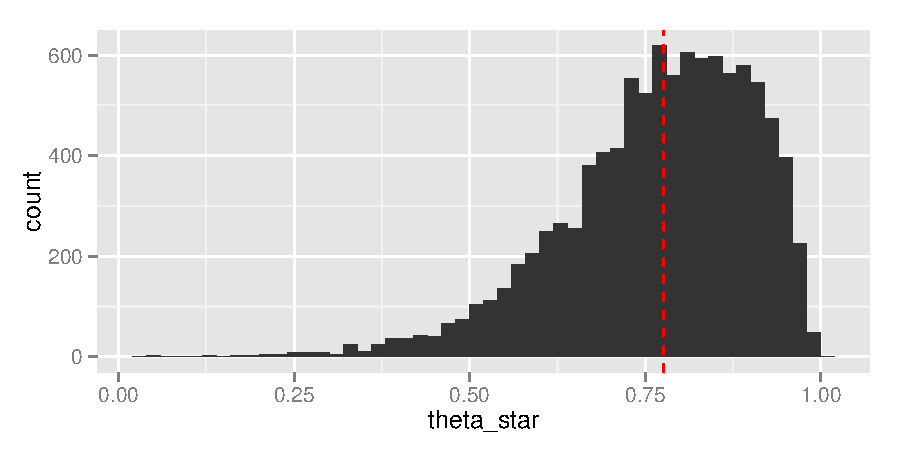
\includegraphics[width=\maxwidth]{figure/chunkname-1} 

\end{knitrout}

\section{Bayesian Bootstrap}
Rubin introduced the Bayesian bootstrap (BB) as the natural Bayesian analogue of the bootstrap. Each BB replication generates a posterior probability for each $x_i$, which is centered at $1/n$, but has variability. To obtain a BB replication, first generate a set of weights by drawing $(n-1)$ uniform(0,1) random variates, $u_1, \ldots, u_(n-1)$, ordering them and calculating the gaps $g_t = u_{(t)} - u_{(t-1)}, t=1,\ldots,n$, where $u_{(0)}=0$ and $u_{(n)}=1$. These gaps, $g = (g_1,\ldots,g_n)$ form the weights to attach to the data values in that replication. Considering all the BB replications gives the BB distribution of $X$, and thus of any parameter of this distibution.\\

Our function BB gives a BB distribution. It takes as its inputs a dataset (as a vector, matrix or dataframe), a function for calculating the statistic $\hat{\theta}$ (this function must take two arguments - one for data and one for weights), and $B$, the number of replications required. It returns a list, the first item of which is the standard error of the replicates. The second item is a dataframe with $\theta_1^*,\ldots,\theta_B^*$.



The following code gives the BB distribution when the parameter of interest is the mean. Here the function weighted.mean is in the R base package.
\begin{knitrout}
\definecolor{shadecolor}{rgb}{0.969, 0.969, 0.969}\color{fgcolor}\begin{kframe}
\begin{alltt}
\hlstd{X} \hlkwb{<-} \hlkwd{rnorm}\hlstd{(}\hlnum{100}\hlstd{,} \hlnum{4}\hlstd{,} \hlnum{2}\hlstd{)}
\hlstd{BB_mean} \hlkwb{<-} \hlkwd{BB}\hlstd{(X, weighted.mean,} \hlkwc{B}\hlstd{=}\hlnum{10000}\hlstd{)}
\hlstd{BB_mean}\hlopt{$}\hlstd{se}
\end{alltt}
\begin{verbatim}
## [1] 0.2037395
\end{verbatim}
\begin{alltt}
\hlkwd{qplot}\hlstd{(T_boot,} \hlkwc{data}\hlstd{=BB_mean}\hlopt{$}\hlstd{replicates,} \hlkwc{geom}\hlstd{=}\hlstr{"histogram"}\hlstd{,} \hlkwc{binwidth}\hlstd{=}\hlnum{0.05}\hlstd{)}
\end{alltt}
\end{kframe}
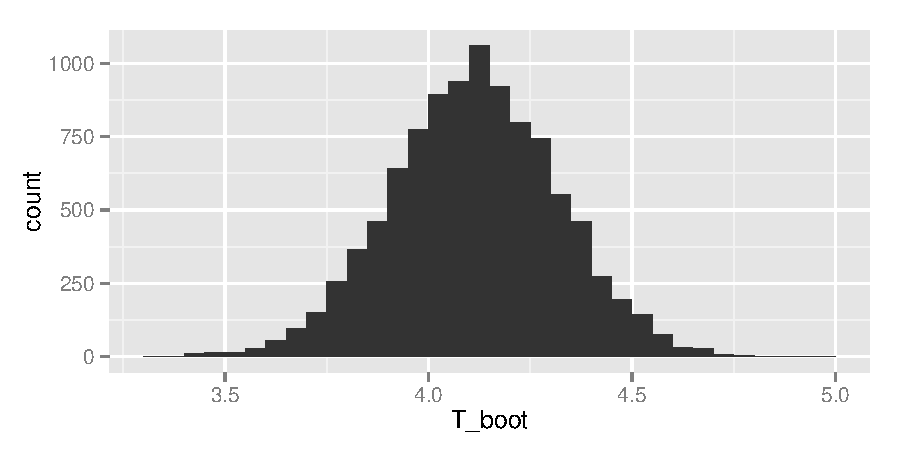
\includegraphics[width=\maxwidth]{figure/unnamed-chunk-2-1} 

\end{knitrout}

It may be necessary to define your own function for the statistic of interest that can take weights as an argument. By may of example, we show the BB equivalent of the correlation example from the previous section.

\begin{knitrout}
\definecolor{shadecolor}{rgb}{0.969, 0.969, 0.969}\color{fgcolor}\begin{kframe}
\begin{alltt}
\hlcom{# takes bivarate data and weights (g) and returns a weighted correlation}
\hlstd{weighted.cor} \hlkwb{<-} \hlkwa{function}\hlstd{(}\hlkwc{data}\hlstd{,} \hlkwc{g}\hlstd{) \{}
  \hlstd{y} \hlkwb{<-} \hlstd{data[,}\hlnum{1}\hlstd{]; z} \hlkwb{<-} \hlstd{data[,}\hlnum{2}\hlstd{]}
  \hlstd{wc_num} \hlkwb{<-} \hlkwd{sum}\hlstd{(g}\hlopt{*}\hlstd{y}\hlopt{*}\hlstd{z)}\hlopt{-}\hlstd{(}\hlkwd{sum}\hlstd{(g}\hlopt{*}\hlstd{y))}\hlopt{*}\hlstd{(}\hlkwd{sum}\hlstd{(g}\hlopt{*}\hlstd{z))}
  \hlstd{wc_den} \hlkwb{<-} \hlstd{(}\hlkwd{sum}\hlstd{(g}\hlopt{*}\hlstd{y}\hlopt{^}\hlnum{2}\hlstd{)}\hlopt{-}\hlstd{(}\hlkwd{sum}\hlstd{(g}\hlopt{*}\hlstd{y))}\hlopt{^}\hlnum{2}\hlstd{)}\hlopt{*}\hlstd{(}\hlkwd{sum}\hlstd{(g}\hlopt{*}\hlstd{z}\hlopt{^}\hlnum{2}\hlstd{)}\hlopt{-}\hlstd{(}\hlkwd{sum}\hlstd{(g}\hlopt{*}\hlstd{z))}\hlopt{^}\hlnum{2}\hlstd{)}
  \hlstd{wc_num}\hlopt{/}\hlkwd{sqrt}\hlstd{(wc_den)}
\hlstd{\}}

\hlkwd{set.seed}\hlstd{(}\hlnum{1}\hlstd{)}
\hlstd{BB_law} \hlkwb{<-} \hlkwd{BB}\hlstd{(law_school, weighted.cor,} \hlkwc{B}\hlstd{=}\hlnum{1000}\hlstd{)}
\hlstd{BB_law}\hlopt{$}\hlstd{se}
\end{alltt}
\begin{verbatim}
## [1] 0.1224361
\end{verbatim}
\begin{alltt}
\hlkwd{qplot}\hlstd{(T_boot,} \hlkwc{data}\hlstd{=BB_law}\hlopt{$}\hlstd{replicates,} \hlkwc{geom}\hlstd{=}\hlstr{"histogram"}\hlstd{,} \hlkwc{binwidth}\hlstd{=}\hlnum{0.02}\hlstd{)}
\end{alltt}
\end{kframe}
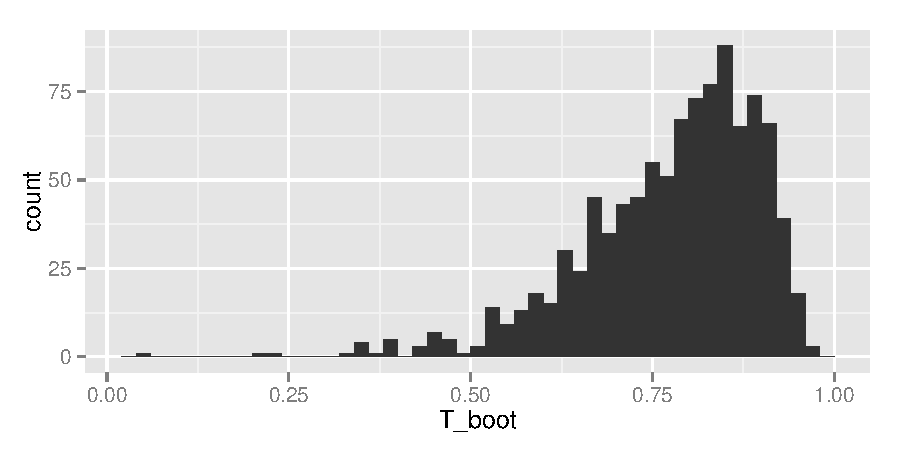
\includegraphics[width=\maxwidth]{figure/unnamed-chunk-3-1} 

\end{knitrout}




ISSUES WITH THE BAYESIAN BOOTSTRAP, AND HENCE BOOTSTRAP.

%Bootstrap methods require



%Boostrap methods encouraged a close relationship between statistical inference and computation and moreover, brought together statistics with computing technology. The latter is very important  has nowadays great importance; firstly because of the increase in the data size and complexity and secondly because of the development of parallel computing architectures. \\ \\


\section{Bag of Little Bootstraps}
The original bootstrap arose around the time when increases in computing power allowed the development of statistical tools that had previously been too computationally expensive. In recent years, there has been an influx of 'big data', alongside the development of parallel computing architectures. CITE KLEINER ET AL have developed a scalable bootstrap for massive data, known as the Bag of Little Bootstraps (BLB). With massive datasets, the bootstrap's need for recomputation on resamples of the same size as the original dataset is problematic. Rather than obtain bootstrap samples from the whole dataset, the BLB breaks down the process as follows:

\begin{enumerate}
\item Repeatedly ($s$ times) subsample $b(n) < n$ points \emph{without replacement} from the original dataset of size $n$.
\item For each of the $s$ subsamples, do the following:
\begin{enumerate}
\item Repeatedly ($r$ times) resample $n$ point \emph{with replacement} from the subsample.
\item Compute $\hat\theta_n^*$ on each resample.
\item Compute an estimate of $\xi$ based on these multiple resampled realisations of $\hat\theta_n^*$.
\end{enumerate}
\item We now have one estimate of $\xi$ per subsample. Output their average as the final estimate of $\xi$ for $\hat\theta_n$.
\end{enumerate}

%by taking $s$ subsamples of the original dataset, each of size $b$, where typically $b \ll n$. Each of these subsamples is generated from the original dataset WITHOUT replacement.


CITE KLEINER recommends taking $b(n) = n^{\gamma}$, where $\gamma \in [0.5,1]$. This procedure dramatically reduces the size of each resample. For example, if $n$ = 1 million and $\gamma=0.6$, the size of the original dataset is around 1TB, with a bootstrap resample typically occupying approximately 632GB, and a BLB subsample or resample occupying just 4GB.


The function BLB.1d implements the simplest version of BLB. It takes as input a 1-dimensional dataset in a vector and a function with computes the statistic of interest, $\theta_n$. It also takes as arguments $s$ and $r$, which default to 20 and 100 respectively (KLEINER demonstates are likely as large as they'll need to be to obtain convergence), and $\gamma$, which controls the value of $b$. The function returns $\xi$, which is set as the standard error.

\begin{knitrout}
\definecolor{shadecolor}{rgb}{0.969, 0.969, 0.969}\color{fgcolor}\begin{kframe}
\begin{alltt}
\hlstd{X} \hlkwb{<-} \hlkwd{rnorm}\hlstd{(}\hlnum{5000}\hlstd{)}
\hlkwd{BLB.1d}\hlstd{(X, mean,} \hlkwc{gamma}\hlstd{=}\hlnum{0.5}\hlstd{)}
\end{alltt}
\begin{verbatim}
## [1] 0.01390571
\end{verbatim}
\end{kframe}
\end{knitrout}

In their paper, CITE KLEINER conduct a simulation study, and here we replicate their results in the Gaussian case. We generate data from the true underlying distribution, a linear model $Y_i = \tilde X_i^{\top}\mathbb{I}_d + \epsilon_i$, with iid $\tilde X_i \sim N(0,1)$ and $\epsilon_i \sim N(0,10)$. The estimator $\hat\theta_n$ consists of a linear least squares regression with a small $L_2$ penalty of $10^{-5}$.

DISCUSSION OF BLB\\
Not run in parallel

\printbibliography
\end{document}
